\documentclass[11pt]{article}
\usepackage[margin=0.7in]{geometry}
\usepackage{multirow}
\usepackage {graphicx}
\usepackage[utf8x]{inputenc} % указать кодировку русского текста
\usepackage[russian]{babel} % указать, что язык текста - русский
\usepackage{fancyhdr}
\pagestyle{fancy}

\begin{document}

\begin{titlepage}

\begin{center}
%\vspace*{1cm}
\large\textbf{Московский Физико-Технический Институт}\\
\large\textbf{(государственный университет)}
\vfill
\line(1,0){430}\\[1mm]
\huge\textbf{Гидрофобные материалы и покрытия}\\
\line(1,0){430}\\[1mm]
\vfill
\large Сибгатуллин Булат, ФРКТ\\
\end{center}

\end{titlepage}

\section*{Введение}\
\indent Традиционно под гидрофобными понимают материалы и покрытия, угол смачивания которых водой и водными растворами превышает $90^{\circ}$. Особенностью таких материалов является неустойчивость тонких смачивающих водных слоев на их поверхностях. Гидрофобность - свойство, которое определяется не столько характеристиками материала в целом, сколько свойствами и структурой приповерхностного слоя толщиной в несколько нанометров.

\indent Практический интерес представляют высокогидрофобные материалы с краевыми углами натекания воды > $120^{\circ}$. Особое место среди таких материалов занимают супергидрофобные материалы и покрытия, характеризующиеся высокими краевыми углами (> $150^{\circ}$) и малым углом наклона поверхности к горизонту, при котором капля воды скатывается (соскальзывает) с поверхности.

\section*{Факторы, определяющие смачивание поверхностей материалов}\

Более двухсот лет назад Т.Юнг впервые рассмотрел и описал силы, действующие на жидкую каплю. В этой работе рассматривалась идеальная, т.е. химически инертная по отношению к тестовой жидкости, гладкая и однородная поверхность (рис. 1,а,б,). Равновесный макроскопический краевой угол $\theta_0$ между мениском объемной жидкости и подложкой определяется соотношением

\begin{equation}
\cos \theta_0 = \frac{\sigma_{sv} - \sigma_{sl}}{\sigma_{lv}},
\end{equation}

где $\sigma_{sv}$ и $\sigma_{sl}$  - поверхностные энергии на границах твердое тело/пар и твердое тело/жидкость, $\sigma_{lv}$ - поверхностное натяжение жидкости. В общем случае $\sigma_{sv}$ отличается от поверхностной энергии на границе твердое тело/вакуум из-за присутствия на поверхности твердого тела тонкой смачивающей/адсорбционной пленки жидкости, находящейся в равновесии с коплей и паром. Анализ соотношения Юнга (1) показал, что гидрофобность можно наблюдать лишь на твердых поверхностях с низкими значениями $\sigma_{sv}$.

\indent С понижением $\sigma_{sv}$ возрастает краевой угол. В качестве иллюстрации такой корреляции в табл. 1 представлены значения поверхностной энергии и краевых углов на гладких поверхностях некоторых материалов.

\vspace{0.5cm}

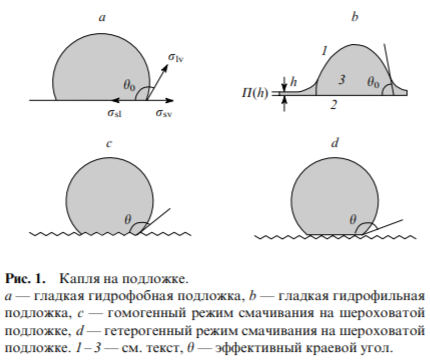
\includegraphics[scale=1.4]{vpv1.png}

\vspace{0.5cm}

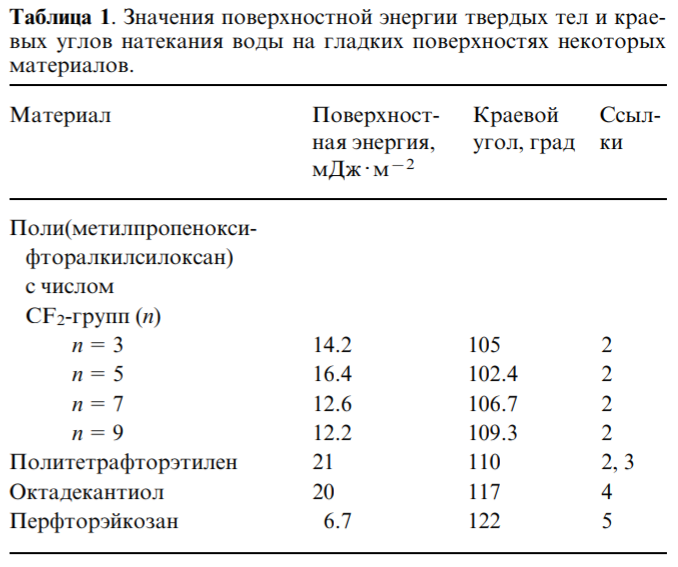
\includegraphics[scale=0.8]{table1.png}

\vspace{0.5cm}

\indent На рис. 2 представлены зависимости краевых углов воды и поверхностной энергии золотой подложки. покрытой монослоем, состоящим из смеси молекул алкантиолов с метильными и карбоксильными концевыми группами, от концентрации гидроксильной компоненты. Монослоя алкантиола с метильными концевыми группами достаточно для придания поверхности гидрофобных свойств.

\vspace{0.5cm}

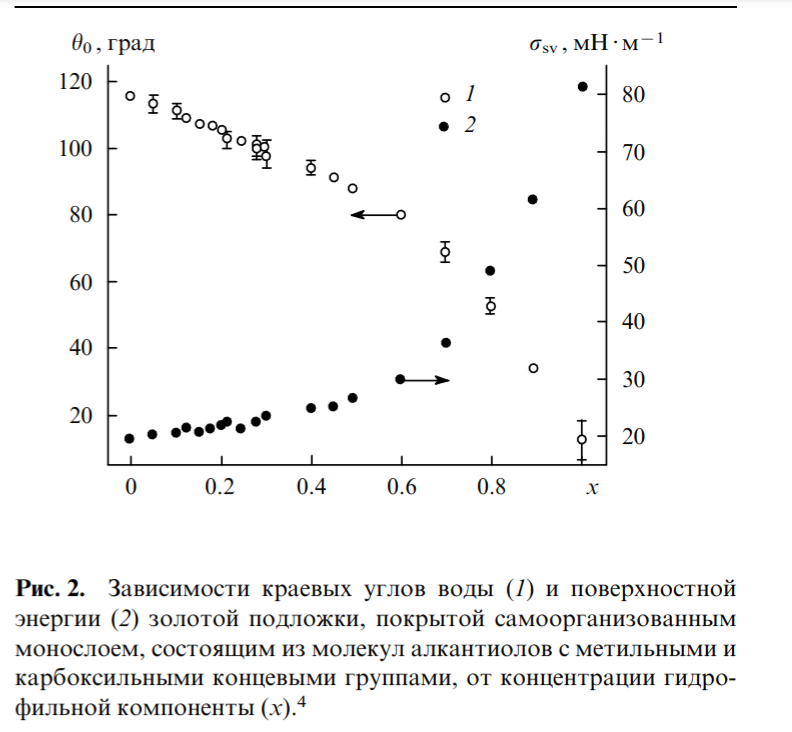
\includegraphics[scale=1]{vpv2.png}

\vspace{0.5cm}

\indent Другой подход к описанию смачивания гладкой однородной поверхности предложен Дерягиным и Фрумкиным. Развитая ими теория смачивания позволяет связать макроскопический краевой угол $\theta_0$ (рис. 1,б) с изотермой расклинивающего давления $\textit{П(h)}$, характеризующей зависимость сил взаимодействия фаз 1 и 2, ограничивающих смачивающую/адсорбционную пленку жидкости 3, от ее толщины \textit{h}

\begin{equation}
\cos \theta_0 = 1 + \frac{1}{\sigma_{lv}}\textit{П(} \textit{h}_e \textit{)h}_e + \frac{1}{\sigma_{lv}}\int\limits_{h_e}^{\infty}\textit{П(h)dh} \approx 1 + \frac{1}{\sigma_{lv}}\int\limits_{h_e}^{\infty}\textit{П(h)dh},
\end{equation}

где $h_e$ - равновесная толщина смачивающей пленки при расклинивающем давлении равном капиллярному давлению в капле. Радиусы кривизны менисков и капель, используемых для экспериментального измерения краевых углов, как правило, находятся в пределах от 1 до 20 мм, что не превышающим 1мПа. В этом случае $h_e$ практически не отличается от толщины $h_0$, соответствующей на изотерме точке с нулевым расклинивающем давлением (рис. 3).

\indent Анализ особенностей трехфазного равновесия показал, что смачивание зависит от вида изотермы расклинивающего давления (рис. 3), который в свою очередь, определяется природой поверхностных сил, действующих в рассматриваемой системе. В случае изотермы типа \textit{1} интеграл будет положительным, следовательно такие трехфазные системы будут характеризоваться полным смачиванием с нулевым краевым углом. Неполному смачиванию отвечают изотермы типа \textit{2} и \textit{3}.

\vspace{0.5cm}

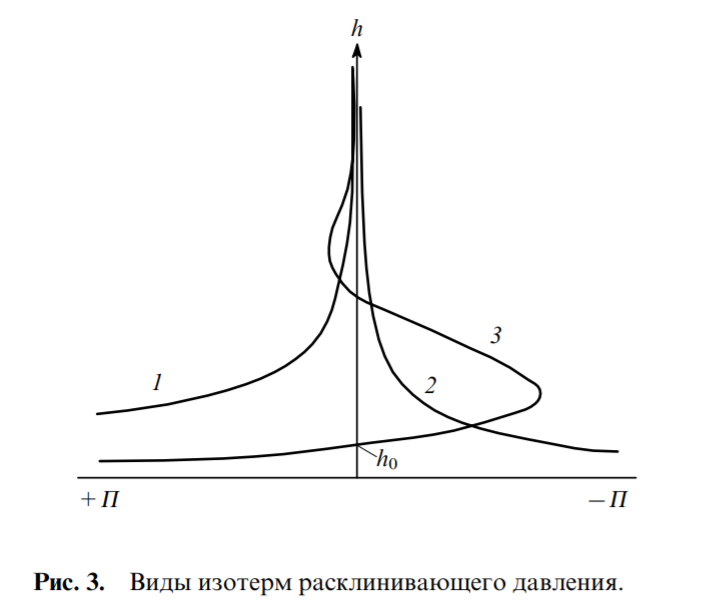
\includegraphics[scale=1]{vpv3.png}

\vspace{0.5cm}

\indent Принципиальное раздичие между системами с двумя последними типами изотерм связано с особенностями смачивания, характеризующего трехфазное равновесие. В системах с изотермой типа \textit{2} $\ll$сидящая$\gg$ капля жидкости будет находиться в равновесии с $\ll$сухой$\gg$ подложкой, свободной от молекул жидкости, в то время как для систем с S-образной изотермой расклинивающего давления (типа \textit{3}) характерно равновесия между каплей и подложкой, покрытой смачивающей/адсорбционной пленкой конечной толщины. Кроме того, значение интеграла в соотношении (2) для систем с изотермой \textit{2} всегда оказывается отрицательным, чем обусловлена отличная от нуля величина краевого угла. Формально большие краевые углы для капель воды на гидрофобных и супергидрофобных поверхностях могут быть достигнуты в системах, характеризуемых как изотермой типа \textit{2}, так и изотермой типа \textit{3}. Необходимым условием здесь является наличие в системе значительных сил притяжения той или иной природы, например структурных.

\end{document}